% Advanced template for the submission to Econometrica journal.
% This template is suggested when *hyperref* package is used.
%
%Author: In this template, the places where you need to add information
%        (or delete line) are indicated by {???}.  Mostly the information
%        required is obvious, but some explanations are given in lines starting
%
%Author:
%All other lines should be ignored.  After editing, there should be
%no instances of ??? after this line.

% use option [draft] for initial submission;
%            [final] for the prepublication;


\documentclass[pdftex]{article}
\usepackage{xspace,amsmath,graphicx,graphics,hypernat,xcolor}
\usepackage{amsthm}
%\startlocaldefs
\newcommand{\etal}{{\it et~al.}\ }
\newcommand{\ie}{{\it i.e.}\ }
\newcommand{\eg}{{\it e.g.}\ }
\newcommand{\etc}{{\it etc.}\ }
\newcommand{\cf}{{\it cf.}\ }
\newcommand{\Ito}{It\^{o}\xspace}
\newcommand{\pa}{{\it p.a.}\xspace}
\newcommand{\psa}{\ensuremath{{\text{year}}^{-1/2}}\xspace}

%List of symbols shortcuts
% For command names that already exist, prepend a "G" (for "Glossary")

\newcommand{\ave}[1]{\left\langle#1 \right\rangle}
\newcommand{\tave}[1]{\overline{#1}}
\newcommand{\latinword}[1]{\textsf{\itshape #1}}
%\newcommand{\person}[1]{{\sc{#1}}}
\newcommand{\person}[1]{#1} % switched off because not used consistently
%\newcommand{\quote}[1]{{\it ``#1''}}
\newcommand{\bi}{\begin{itemize}}
\newcommand{\ei}{\end{itemize}}

\newcommand{\elabel}[1]{\label{eq:#1}}
\newcommand{\eref}[1]{(Eq.~\ref{eq:#1})}
\newcommand{\Eref}[1]{Equation~(\ref{eq:#1})}

\newcommand{\ceref}[2]{(\ref{eq:#1}#2)}

\newcommand{\tlabel}[1]{\label{tab:#1}}
\newcommand{\tref}[1]{Table~\ref{tab:#1}}

\newcommand{\flabel}[1]{\label{fig:#1}}
\newcommand{\fref}[1]{Fig.~\ref{fig:#1}}
\newcommand{\Fref}[1]{Figure ~\ref{fig:#1}}

\newcommand{\seclabel}[1]{\label{section:#1}}
\newcommand{\secref}[1]{Sec.~\ref{section:#1}}
\newcommand{\Secref}[1]{Section~\ref{section:#1}}

\newcommand{\clabel}[1]{\label{chapter:#1}}
\newcommand{\cref}[1]{Chap.~\ref{chapter:#1}}
\newcommand{\Cref}[1]{Chapter~\ref{chapter:#1}}



\newcommand{\OP}[1]{{\bf @@@OP: #1 @@@}}
\renewcommand{\AA}[1]{{\bf ===AA: #1 ===}}

\newcommand{\eq}{\hspace{-.15cm}=\hspace{-.15cm}}
\newcommand{\dist}{\,{\buildrel d \over =}\,}
\newcommand{\be}{\begin{equation}}
\newcommand{\ee}{\end{equation}}
\newcommand{\bea}{\begin{eqnarray}}
\newcommand{\eea}{\end{eqnarray}}
\newcommand{\bc}{\begin{center}}
\newcommand{\ec}{\end{center}}
\newcommand{\prob}[1]{\mathcal{P}\left(#1\right)}
\newcommand{\DW}{{\Delta W}}
\newcommand{\Dx}{{\Delta x}}
\newcommand{\DX}{{\Delta X}}
\newcommand{\Du}{\Delta u}
\newcommand{\tm}{{f_{\text{\normalfont{m}}}}}
\newcommand{\tml}{{f_{\text{\normalfont{m}}}^{\text{\normalfont{U}}}}}
\newcommand{\tmb}{{f_{\text{\normalfont{m}}}^{\text{\normalfont{B}}}}}
\newcommand{\dW}{{\delta W}}
\newcommand{\gbar}{\bar{g}}
\newcommand{\nn}{\nonumber}

% load additional packages:
%\usepackage{amsthm,amsmath,natbib}
%\RequirePackage[colorlinks,citecolor=blue,urlcolor=blue]{hyperref}

% use this package if hyperref and natbib is used:
%\RequirePackage{hypernat}

% put your definitions there:
%\endlocaldefs

\begin{document}

%\begin{frontmatter}

% "Title of the paper"
\title{Comment on D. Bernoulli (1738)}
\author{Ole Peters\\
\\
{\small London Mathematical Laboratory, 8 Margravine Gardens, London W6 8RH, UK}\\
{\small Santa Fe Institute, 1399 Hyde Park Road, Santa Fe, 87501 NM, USA}\\
{\small o.peters@lml.org.uk}}
\maketitle

%\runauthor{O. Peters}


\begin{figure}
\centering
\begin{picture}(300,200)(0,0)
  \put(-55,0){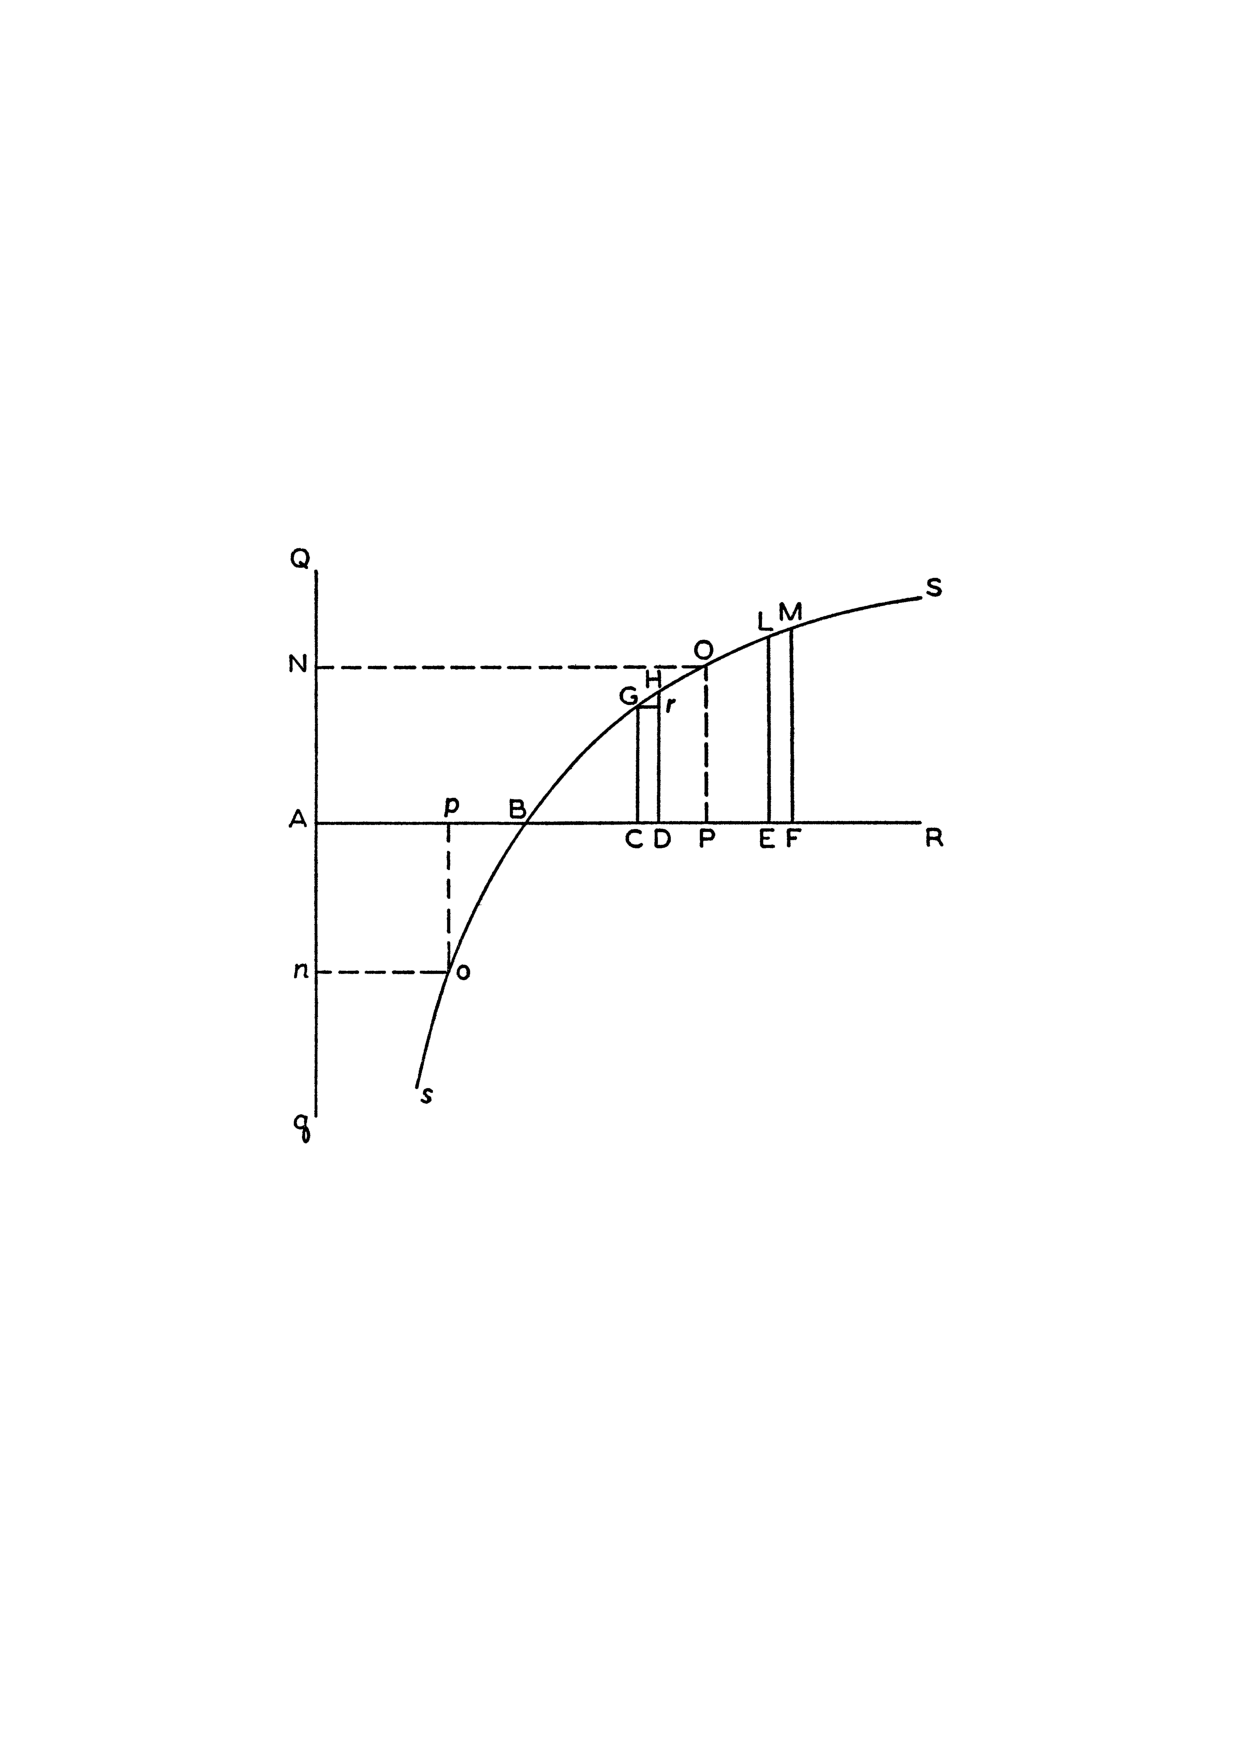
\includegraphics[width=.89\textwidth]{./Bernoulli1738.pdf}}
\put(-55,245){\colorbox{white}{Utility $u(x)$}}
\put(-54,137){\colorbox{white}{$u(x_0)$}}
\put(-89,199.5){\colorbox{white}{$\mathbin{{u(x_0)}{+}{\ave{\Du^+}}}$}}
\put(-83,77){\colorbox{white}{$\mathbin{{u(x_0)}{-}{\Du^-}}$}}
%delete q
\put(-33,19){\colorbox{white}{~}}
\put(-31,16){\colorbox{white}{~}}
\put(-31,12){\colorbox{white}{~}}
%delete s
\put(20,30){\colorbox{white}{~}}
\put(18,25){\colorbox{white}{~}}
%delete o
\put(34,80){\colorbox{white}{~}}
\put(34,75){\colorbox{white}{~}}
%delete C,D,P,E,F,R
\put(90,134){\colorbox{white}{\hspace{5cm}}}
\put(90,130){\colorbox{white}{\hspace{5cm}}}
%delete G
\put(98.5,192){\colorbox{white}{~}}
\put(98.5,190){\colorbox{white}{~}}
\put(98,189.5){\colorbox{white}{~}}
\put(96.5,188.5){\colorbox{white}{~}}
%delete H
\put(108,197.7){\colorbox{white}{~}}
\put(107.5,195.6){\colorbox{white}{~}}
%delete r
\put(118,189){\colorbox{white}{~}}
\put(118,185){\colorbox{white}{~}}
%delete O
\put(128.5,207.5){\colorbox{white}{~}}
\put(128.5,211){\colorbox{white}{~}}
\put(127,206.7){\colorbox{white}{~}}
%delete L
\put(154,221){\colorbox{white}{~}}
\put(154,218.5){\colorbox{white}{~}}
%delete M
\put(163,227){\colorbox{white}{~}}
\put(163,222){\colorbox{white}{~}}
\put(165,228){\colorbox{white}{~}}
\put(164,223){\colorbox{white}{~}}
%delete S
\put(222.2,235){\colorbox{white}{~}}
\put(222.2,230){\colorbox{white}{~}}
\put(8,145){\colorbox{white}{$\mathbin{{x_0}{-}{\tmb}}$}}
\put(53.3,143.2){\colorbox{white}{~}}
\put(53.5,146.3){\colorbox{white}{~}}
\put(54,144.5){$x_0$}
\put(126,127){\colorbox{white}{$\mathbin{{x^+}}$}}
\put(68,110){\colorbox{white}{$\mathbin{{x_0}{+}{\pi_1}}$}}
\put(87,119){\vector(1,1){16}}
\put(88,95){\colorbox{white}{$\mathbin{{x_0}{+}{\pi_2}}$}}
\put(105,105){\vector(1,3){10}}
\put(177,110){\colorbox{white}{$\mathbin{{x_0}{+}{\pi_4}}$}}
\put(189,119){\vector(-1,1){16}}
\put(155,95){\colorbox{white}{$\mathbin{{x_0}{+}{\pi_3}}$}}
\put(171,105){\vector(-1,3){10}}
\put(230,137){\colorbox{white}{Wealth $x$}}
\end{picture}
%\caption{\small A) Figure representing Bernoulli's 1738 computation of the maximum fee to be paid for a lottery. B) the same figure translated into modern notation. In Bernoulli's EUT, unlike in modern EUT, the maximum fee to be paid for a gamble is found as follows: find 1) the gain in utility, $\Du^+$ that would arise from receiving the expectation value of the prize (disregarding the fee). Find 2) the fee such that the loss in utility that would arise from paying it without receiving any prize, $\Du^-$ is the same as $\Du^+$. This contradicts modern utility theory where the maximum fee is the fee that renders the expectation value of the change in utility due to net changes in wealth zero, $\ave{\Du}=0$.}
%\flabel{key}
\end{figure}
%
\begin{figure}
\centering
\begin{picture}(300,500)(0,0)
  \put(-10,200){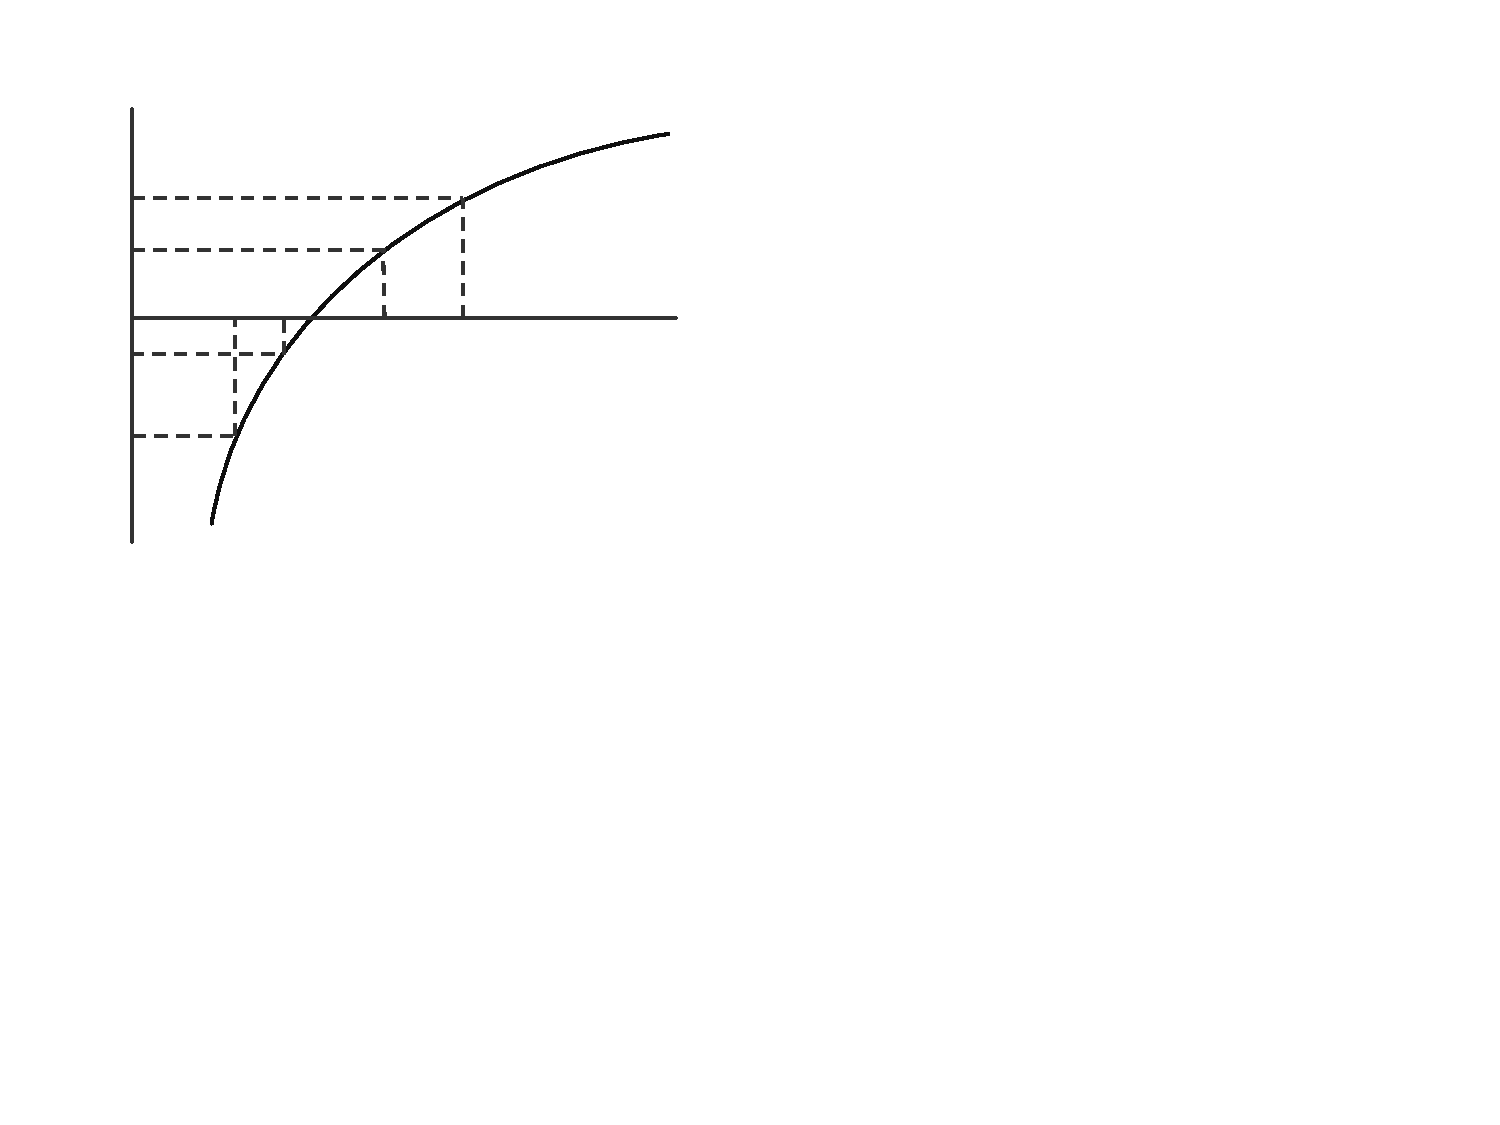
\includegraphics[width=1.12\textwidth]{./EUT_curve.pdf}}
 \put(40,360){$\mathbin{{x_0}{+}{\Dx_1}}$}
 \put(85,360){$\mathbin{{x_0}{+}{\Dx_2}}$}
 \put(120,345){$x_0$}
 \put(150,345){$\mathbin{{x_0}{+}{\Dx_3}}$}
 \put(210,345){$\mathbin{{x_0}{+}{\Dx_4}}$}
 \put(-55,435){$\mathbin{{u(x_0}{+}{\Dx_4)}}$}
 \put(-55,400){$\mathbin{{u(x_0}{+}{\Dx_3)}}$}
 \put(-88,355){$\mathbin{{u(x_0)}{=}{\ave{u(\mathbin{{x_0}{+}{\Dx)}}}}}$}
 \put(-55,330){$\mathbin{{u(x_0}{+}{\Dx_2)}}$}
 \put(-55,275){$\mathbin{{u(x_0}{+}{\Dx_1)}}$}
 \put(10,485){Utility $u(x)$}
 \put(330,365){Wealth $x$}
\end{picture}
\caption{Modern EUT.}
\flabel{key}
\end{figure}



\bibliographystyle{plain}
\bibliography{bibliography}
\end{document}

